Action potentials in electrophysiological systems are very low amplitude in the order of $10\unit{\mu V}$ to $100\unit{\mu V}$~\cite{Potter2005}.  To study the electrophysiological signals with electrical equipment, the first step is to amplify the low voltage action potentials.  Previous work on this has been done in the Neurobiology Engineering Laboratory yielding a low noise amplifier design~\cite{StahlMSEE,BatzerCorsiCrampton}.  Since then, the design has been adapted to fit on a PCB with a card edge connector compatible with 36-pin connectors designed for PCI-Express cards but with a custom pinout.  This approach allows the tested Preamp design to be built independently of the rest of the experimental system, and eliminates the need to replicate the sensitive circuit that can be susceptible to noise.  Pictures of the card edge connector version of the Preamp board, provided by John Stahl, are shown in Figure~\ref{fig:PreampBoard}.

\begin{figure}[h]
	\centering 
	\begin{singlespace}
	\begin{subfigure}[b]{\textwidth}
		\centering 
		\includegraphics{./figures/PreAmpTop} 
	\caption{Top side\label{fig:patop}}
	\end{subfigure}
	\\
	\begin{subfigure}[b]{\textwidth}
		\centering 
		\includegraphics{./figures/PreAmpBot} 
	\caption{Bottom Side\label{fig:pabot}}
	\end{subfigure}
	\caption{Views of a populated Preamp Board with card edge connector, provided by John Stahl\label{fig:PreampBoard}}
	\end{singlespace}
\end{figure}

A block diagram of the Preamp board, based on~\cite{Jimbo2003,StahlMSEE}, is shown in Figure~\ref{fig:PreampInt} along with its connection to the Electrophysiology Interface board.  Not shown is the analog power and ground connections to the Preamp.  A summary of the connections is shown in Table~\ref{tab:PreampInt}.

\begin{figure}[h!]
	\centering 
		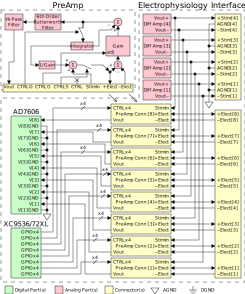
\includegraphics{./figures/PreAmpInt} 
	\caption{Preamp block diagram~\cite{Jimbo2003, StahlMSEE} and Electrophysiology Interface board connections\label{fig:PreampInt}}
\end{figure}

\renewcommand{\arraystretch}{1.3}
\begin{table}[h]
\centering 
\begin{tabular}{|l|l|p{3.5in}|}
\hline
Signal	&	Connector Pin	& Function\\
\hline
+Elect	& B4	& Non-inverting input of low-noise instrumentation amplifier\\
\hline
$-\mathrm{Elect}$	& B2	& Inverting input of low-noise instrumentation amplifier\\
\hline
StimIn	& A13	& Single-ended stimulation input that can be routed to the non-inverting input\\
\hline
Vout	& B13	& Single-ended output of the Preamp\\
\hline
CTRLO	& A15	& Digital input controls AC coupling integrator\\
\hline
CTRLS	& A16	& Digital input controls connecting summing amplifier to non-inverting input\\
\hline
CTRLG	& A17	& Digital input controls gain of instrumentation amplifier\\
\hline
CTRL	& A18	& Digital input controls unused analog switch.  Included for any future design needs\\
\hline
V+	& B10	& Positive analog voltage supply for Preamp circuits.  Connected to +VA supply on Electrophysiology Interface board\\
\hline
$\mathrm{V}-$	& B8	& Negative analog voltage supply for Preamp circuits.  Connected to $-\mathrm{VA}$ supply on Electrophysiology Interface board\\
\hline
GND	& All others	& Remaining pins on connector are used to connect to circuit ground.  Connected to AGND on Electrophysiology Interface board \\
\hline
\end{tabular}
\caption{Preamp PCI-Express 36-pin connector signals and pinout\label{tab:PreampInt} }

\end{table}
\renewcommand{\arraystretch}{1.0}

The Preamp consists of a differential input that is connected to the recording electrodes of the biological system.  The low voltage signal from the electrodes is amplified by a low-noise instrumentation amplifier.  An integrator connected to the instrumentation amplifier subtracts the DC part of the signal which is then passed to a 6th Order Butterworth Filter for additional gain and bandwidth reduction.  A high-pass filter removes any DC component added by the Butterworth Filter circuit, and the result is a single ended output signal.

The Preamp also has the capability of outputting a stimulation signal on the non-inverting electrode with the DC offset of the electrode added to the stimulation signal~\cite{Jimbo2003,StahlMSEE}.  Four digital control signals, with one not used by the Preamp, connected to analog switches and a stimulation input are needed to realize this function.  CTRLO disconnects the integrator from the instrumentation amplifier output so the stimulation signal does not affect the DC offset calculation; CTRLG reduces the gain of the instrumentation amplifier to keep the amplifier from saturating when the comparatively high voltage stimulation signal is added to the electrode; an op-amp circuit adds the DC offset value, which is the integrator output divided by the instrumentation amplifier gain, to the single-ended stimulation signal, StimIn; and, finally, CTRLS connects the summing op-amp to the non-inverting electrode.  The stimulation signal overpowers any biological signals on the recording electrode and allows an artificial signal to be applied to a biological system.  

A summary of the digital signals that control the Preamp stimulation mode is in Table~\ref{tab:PreampStim}.  Pull-up and pull-down resistors are included on the Preamp board to default its behavior to measurement mode.  Tri-stated outputs may be connected to the Preamp's digital inputs for measurement mode.  Additional work may be needed to determine the optimal relative timing of the signals for switching modes~\cite{StahlMSEE}.

\renewcommand{\arraystretch}{1.3}
\begin{table}[hb]
\centering 
\begin{tabular}{|l|l|l|}
\hline
Signal	&	Measurement	& Stimulation\\
\hline
CTRLO	& HIGH or tri-state	& LOW\\
\hline
CTRLS	& LOW or tri-state	& HIGH\\
\hline
CTRLG	& LOW or tri-state	& HIGH\\
\hline
CTRL	& X	& X\\
\hline
\end{tabular}
\caption{Preamp digital control for stimulation mode\label{tab:PreampStim} }

\end{table}
\renewcommand{\arraystretch}{1.0}

A summary of how the Electrophysiology Board is connected to the Preamp, as shown in Figure~\ref{fig:PreampInt}, is now provided. A terminal block connects the biological system measurement electrodes to the Preamp electrode inputs.  Differential or single-ended stimulation signals from the four Differential Output Amplifiers may be connected to the biological system using a terminal block, or the single-ended stimulation signals may be routed to the non-inverting recording electrodes by changing the desired Preamp to stimulation mode.  The output of the Preamps are connected to the analog inputs of the AD7606 ADC.  Not shown in the figure are $0\unit{\Omega}$ resistors that may be used to bypass the Preamp by connecting the non-inverting electrode signal from the terminal block to the input of the ADC (this should only be done when a Preamp board is not in the PCI-Express connector).  A $0\unit{\Omega}$ resistor can also be used to connect the inverting input of the Preamps to AGND.  A Xilinx\textsuperscript{\textregistered} XC9572XL CPLD (or the pin-compatible XC9536XL) connects to all of the control inputs of the Preamps.
